Here is all the stuff of the analysis!

\section{Final state particle}
	-final state particle: proton, antiproton, \piminus, \piplus, \kminus and \kplus mesons
	-reconstructed in Detector
	-only particles with more then 3 hits either in one of the subdetectors (reason: 3 hits define circle; fourth hit point gives a validation for track hypothesis)
	- ideal PID (reason!!!)
		
	\begin{figure}
		\centering
		
		\caption{The plot is showing the number of reconstructed particles...}
		\label{fig:finalstate_allparticles}
	\end{figure}
	
	-reco efficiency in table \ref{tab:finalstate_recoeff}
	
	\begin{table}
		\centering
		\caption{reco efficiency and momentum resolution}
		\label{tab:finalstate_recoeff}
		\begin{tabular}{lll}
			\hline
			final state & N/$\%$ & $\frac{\sigma p}{p}/\%$ \\
			\hline
			\hline
			\piminus &  & \\
			\piplusone(\anticascade) &  & \\
			\piplustwo(\alam) &  &\\
			\kminus&  &\\
			p &  &\\
			\antiproton &  &\\\hline
			 
		\end{tabular}
	\end{table}
	

	
\section{Reconstruction of $\boldmath{\Lambda}^0$ and $\boldmath{\bar{\Lambda}^0}$}
	\subsection{Combination}
		-only final state particle with more than 3 Hits
		
		-daughter particles for \lam: proton an \piminus meson
		
		-daughter particles for \alam: \antiproton and \piplus here \piplus2 
		
		-fitting daughters to common point using kinematic vertex fitter
		
		-using mass fitter with input of vertex fitter 
		
		-only select particles with prob bigger than 0.01 for both fitter
		
		-scheme in figure \ref{fig:lambda_scheme}
		
		\begin{figure}
			\centering
				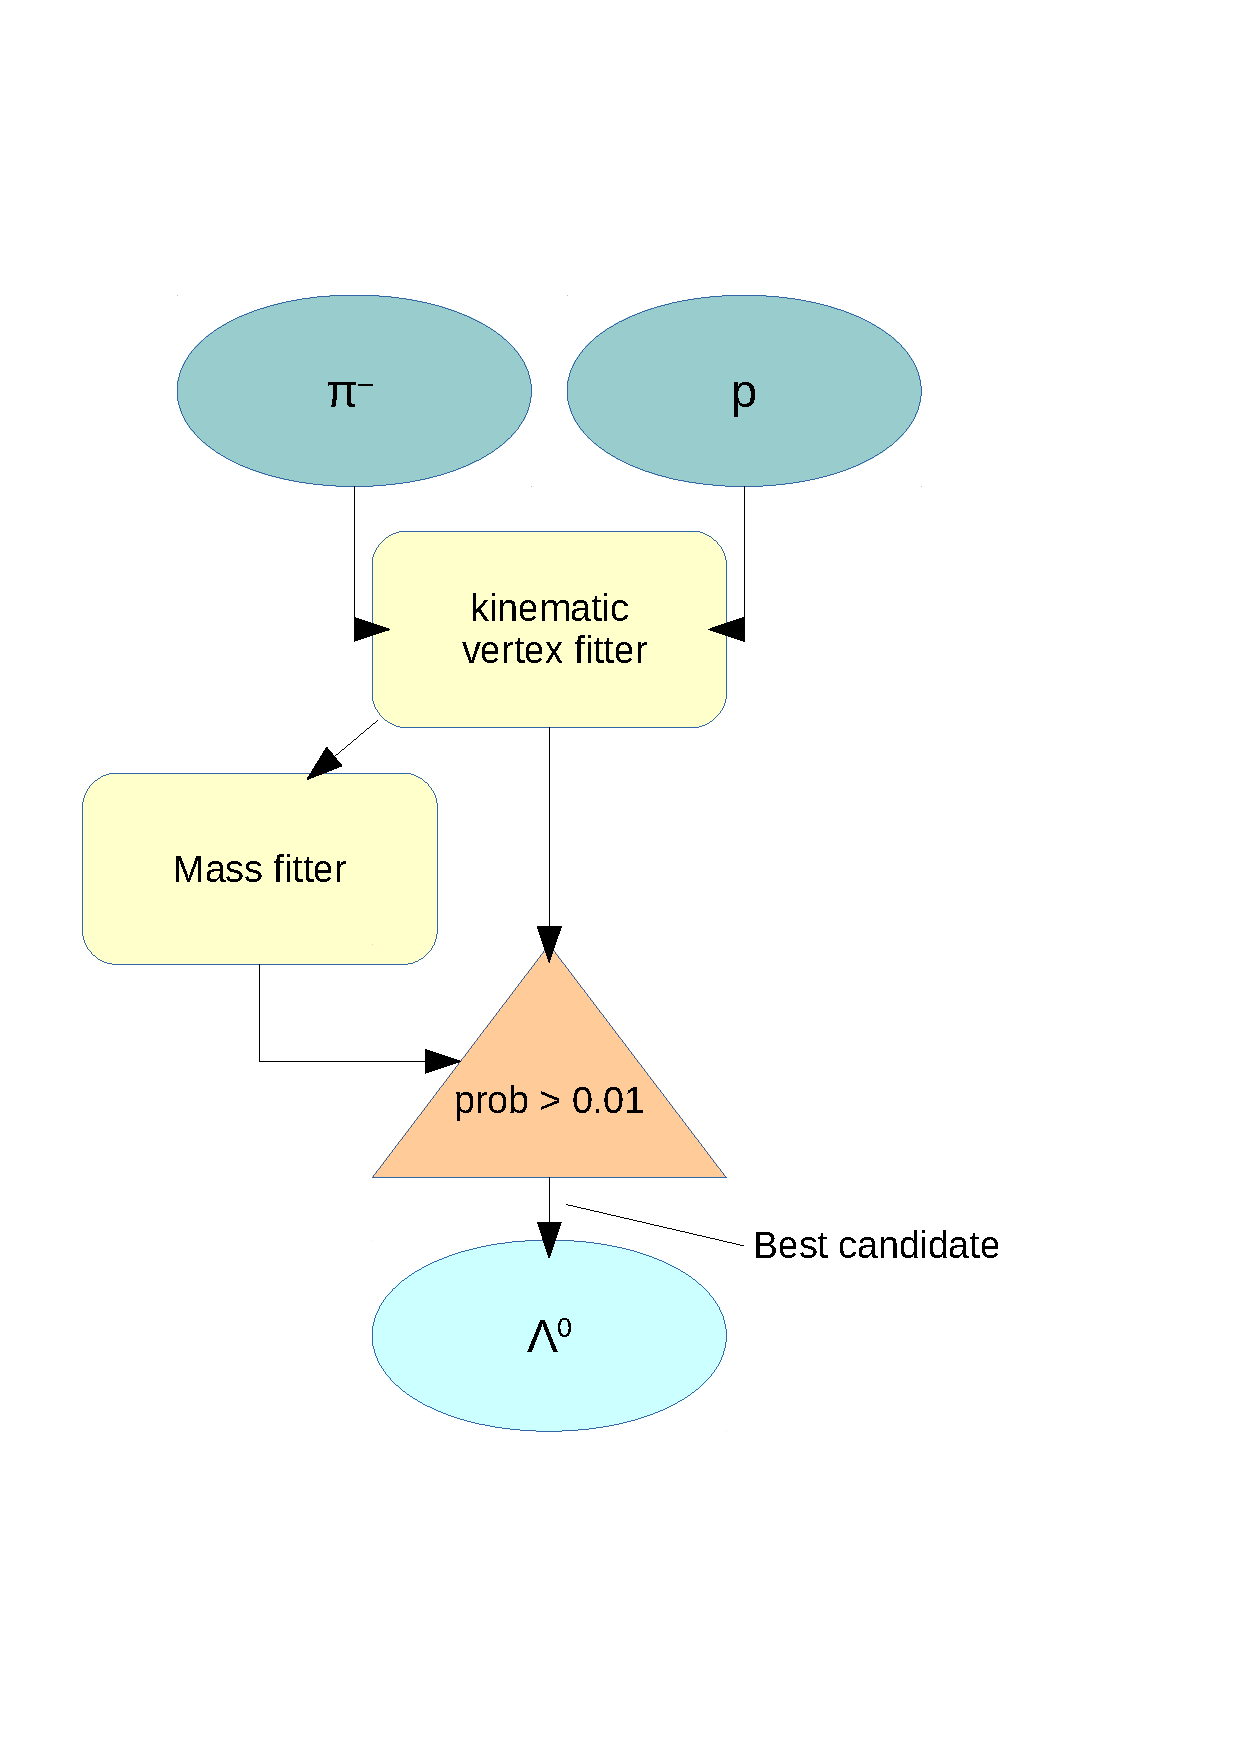
\includegraphics[width=0.50\textwidth]{C:/Users/Guinivere/Documents/GitHub/PhD/ReleaseNote/plots/combineLambda0.pdf}
			\caption{Scheme for \lam reconstruction}
			\label{fig:lambda_scheme}
		\end{figure}
		
		-if there is more than one particle choose best candidate to go on
		
	\subsection{Fitting}
	
\section{Reconstruction of $\boldmath{\Xi}$ and $\boldmath{\bar{\Xi}}$}
	\subsection{Combination}
	\subsection{Fitting}

\section{Reconstruction of $\boldmath{\Xi}$(1820) and $\boldmath{\bar{\Xi}}$(1820)}
	\subsection{Combination}
	\subsection{Fitting}
	
\section{Reconstruction of hole chain}